% !TEX program = pdflatex
% !TEX options = -synctex=1 -interaction=nonstopmode -file-line-error "%DOC%"
% 固体物理第七次作业
\documentclass[UTF8,10pt,a4paper]{article}
\usepackage{ctex}
% \catcode`\。=\active
% \newcommand{。}{.}
\newcommand{\CourseName}{固体物理}
\newcommand{\CourseCode}{PHYS1502}
\newcommand{\Semester}{2019-2020学年第二学期}
\newcommand{\ProjectName}{第七次作业}
\newcommand{\DueTimeType}{截止时间}
\newcommand{\DueTime}{2020. 4. 24(周五)17:00}
\newcommand{\StudentName}{陈稼霖}
\newcommand{\StudentID}{45875852}
\usepackage[vmargin=1in,hmargin=.5in]{geometry}
\usepackage{fancyhdr}
\usepackage{lastpage}
\usepackage{calc}
\pagestyle{fancy}
\fancyhf{}
\fancyhead[L]{\CourseName}
\fancyhead[C]{\ProjectName}
\fancyhead[R]{\StudentName}
\fancyfoot[R]{\thepage\ / \pageref{LastPage}}
\setlength\headheight{12pt}
\fancypagestyle{FirstPageStyle}{
    \fancyhf{}
    \fancyhead[L]{\CourseName\\
        \CourseCode\\
        \Semester}
    \fancyhead[C]{{\Huge\bfseries\ProjectName}\\
        \DueTimeType\ : \DueTime}
    \fancyhead[R]{姓名 : \makebox[\widthof{\StudentID}][s]{\StudentName}\\
        学号 : \StudentID\\
        成绩 : \underline{\makebox[\widthof{\StudentID}]{}}}
    \fancyfoot[R]{\thepage\ / \pageref{LastPage}}
    \setlength\headheight{36pt}
}
\usepackage{amsmath,amssymb,amsthm,bm}
\allowdisplaybreaks[4]
\newtheoremstyle{Problem}
{}
{}
{}
{}
{\bfseries}
{.}
{ }
{第\thmnumber{ #2}\thmname{ #1}\thmnote{ (#3)} 得分: \underline{\qquad\qquad}}
\theoremstyle{Problem}
\newtheorem{prob}{题}
\newtheoremstyle{Solution}
{}
{}
{}
{}
{\bfseries}
{:}
{ }
{\thmname{#1}}
\makeatletter
\def\@endtheorem{\qed\endtrivlist\@endpefalse}
\makeatother
\theoremstyle{Solution}
\newtheorem*{sol}{解}
\usepackage{graphicx}
\begin{document}
\thispagestyle{FirstPageStyle}
\begin{prob}[(12.2) Neighbor in the Face-Centered Lattice.]
    \begin{enumerate}
        \item[(a)] Show that each lattice point in an fcc lattice has twelve nearest neighbors, each the same distance from the initial point. What is the distance if the conventional unit cell has lattice constant $a$?
        \item[(b)$^*$] Now sketch the side lengths of the fcc lattice such that you obtain a face-centered orthorhombic lattice where the conventional unit cell has sides of length $a$, $b$, $c$ which are all different. What are the distances to these twelve neighboring points now? How many nearest neighbors are there?
    \end{enumerate}
\end{prob}
\begin{sol}
    \begin{enumerate}
        \item[(a)] fcc的基元只包含一个原子,故只需对其晶格中一个原子证明其周围有$12$个最近的、距离相同的原子即可. 如图\ref{1-fcc},用fcc传统晶胞的基矢表示原子坐标,以$[0,0,0]$处的原子为例(图中标号为0). 其余标号的$12$个原子即为与之最近的、距离相同的原子,其坐标如表\ref{1-fcc-T}. 这些最近原子到标号为0的原子的距离均为$\frac{a}{\sqrt{2}}$.
        \begin{figure}[h]
            \centering
            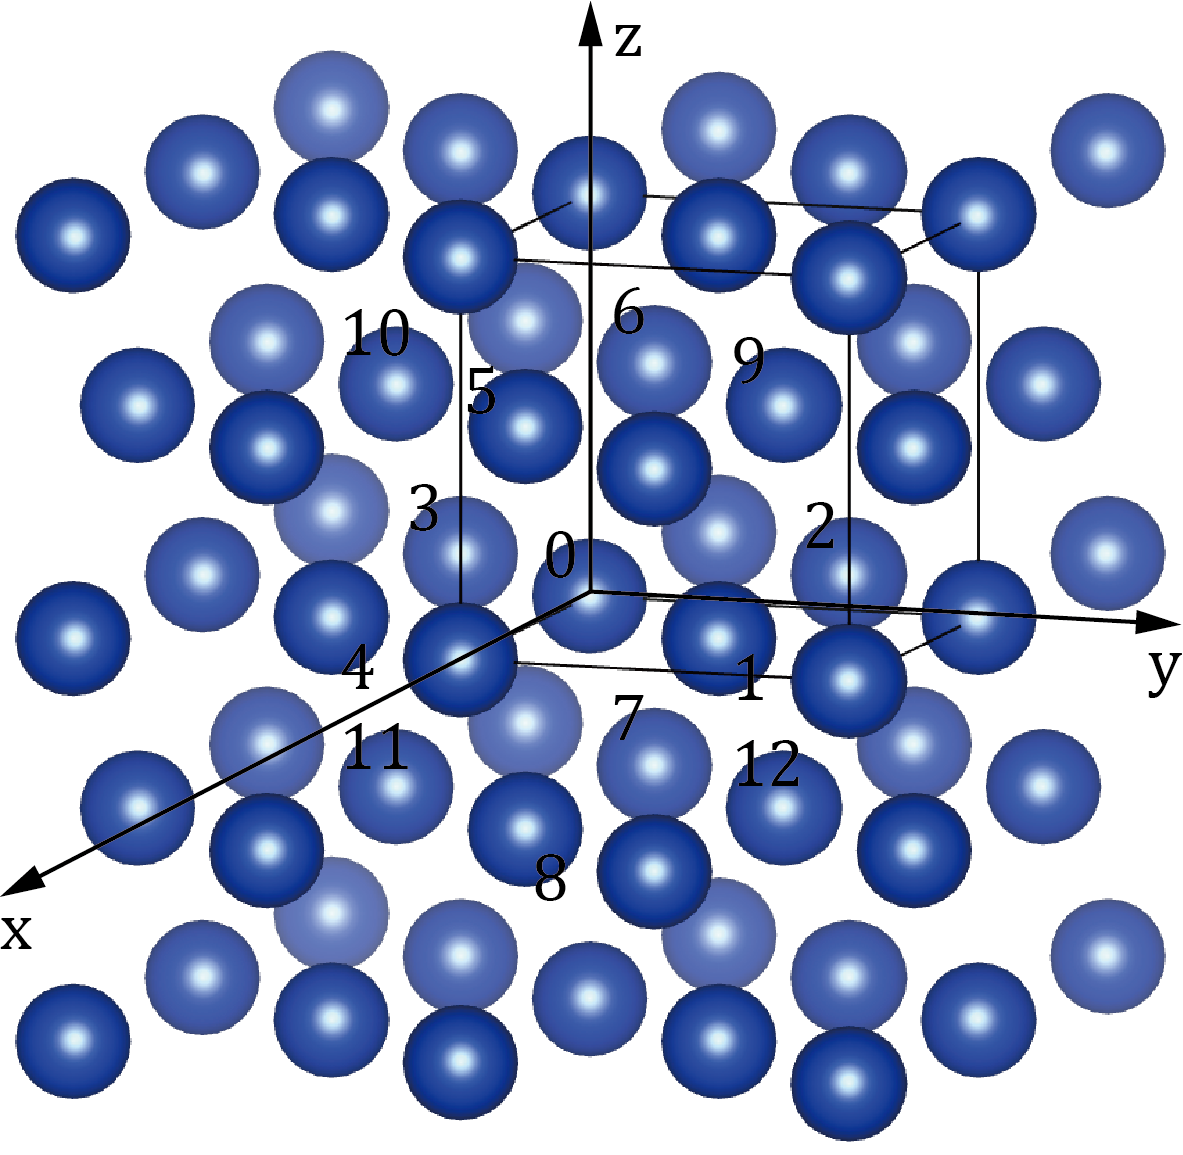
\includegraphics[width=.32\textwidth]{1-fcc-2.png}
            \caption{fcc晶格.}
            \label{1-fcc}
        \end{figure}
        \begin{table}[h]
            \caption{邻近原子标号和坐标.}
            \label{1-fcc-T}
            \begin{tabular}{c|cccccccc}
            标号 & 1 & 2 & 3 & 4 & 5 & 6 & 7 & 8 \\ \hline
            坐标 & $[\frac{1}{2},\frac{1}{2},0]$ & $[-\frac{1}{2},\frac{1}{2},0]$ & $[-\frac{1}{2},-\frac{1}{2},0]$ & $[\frac{1}{2},-\frac{1}{2},0]$ & $[\frac{1}{2},0,\frac{1}{2}]$ & $[-\frac{1}{2},0,\frac{1}{2}]$ & $[-\frac{1}{2},0,-\frac{1}{2}]$ & $[\frac{1}{2},0,-\frac{1}{2}]$
            \end{tabular}
            \begin{tabular}{c|cccc}
                标号 & 9 & 10 & 11 & 12 \\ \hline
                坐标 & $[0,\frac{1}{2},\frac{1}{2}]$ & $[0,-\frac{1}{2},\frac{1}{2}]$ & $[0,-\frac{1}{2},-\frac{1}{2}]$ & $[0,\frac{1}{2},-\frac{1}{2}]$
                \end{tabular}
        \end{table}
        \item[(b)] 如图\ref{1-fcc-2},沿用上一小题中的标号,当三个晶格常数$a\neq b$,$b\neq c$,$c\neq a$时,标号1,2,3,4的原子到标号为0的原子的距离为$\frac{1}{2}\sqrt{a^2+b^2+c^2}$,标号为5,6,7,8的原子到标号为0的原子距离为$\frac{1}{2}\sqrt{a^2+c^2}$,标号为9,10,11,12的原子到标号为0的原子的距离为$\frac{1}{2}\sqrt{b^2+c^2}$. 此时离标号为0的原子最近的原子只有$4$个.
        \begin{figure}[h]
            \centering
            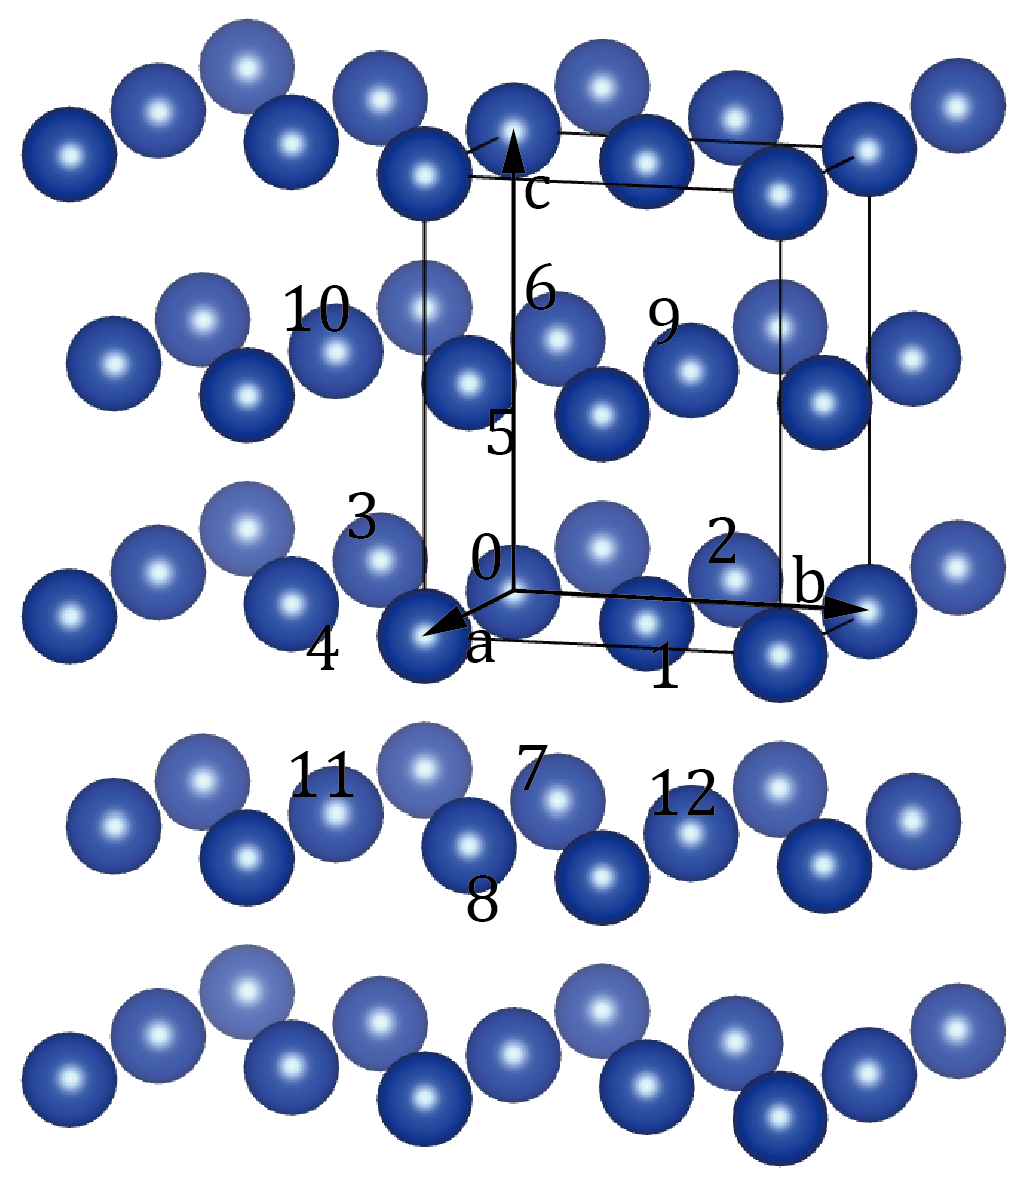
\includegraphics[width=.32\textwidth]{1-fcc-4.png}
            \caption{fcc正交晶系.}
            \label{1-fcc-2}
        \end{figure}
    \end{enumerate}
\end{sol}

\begin{prob}[(12.3) Crystal Structure]
    The diagram of Fig. \ref{2} shows a plan view of a structure of cubic ZnS (zincblende) looking down the $z$ axis. The number attached to some atoms represent the heights of the atoms above the $z=0$ plane expressed as a fraction of the cube edge $a$.
    \begin{enumerate}
        \item[(a)] What is the Bravais lattice type?
        \item[(b)] Describe the basis.
        \item[(c)] Given that $a=0.541$ nm, calculate the nearest-neighbor Zn-Zn, Zn-S, and S-S distances.
    \end{enumerate}
    \begin{figure}[h]
        \centering
        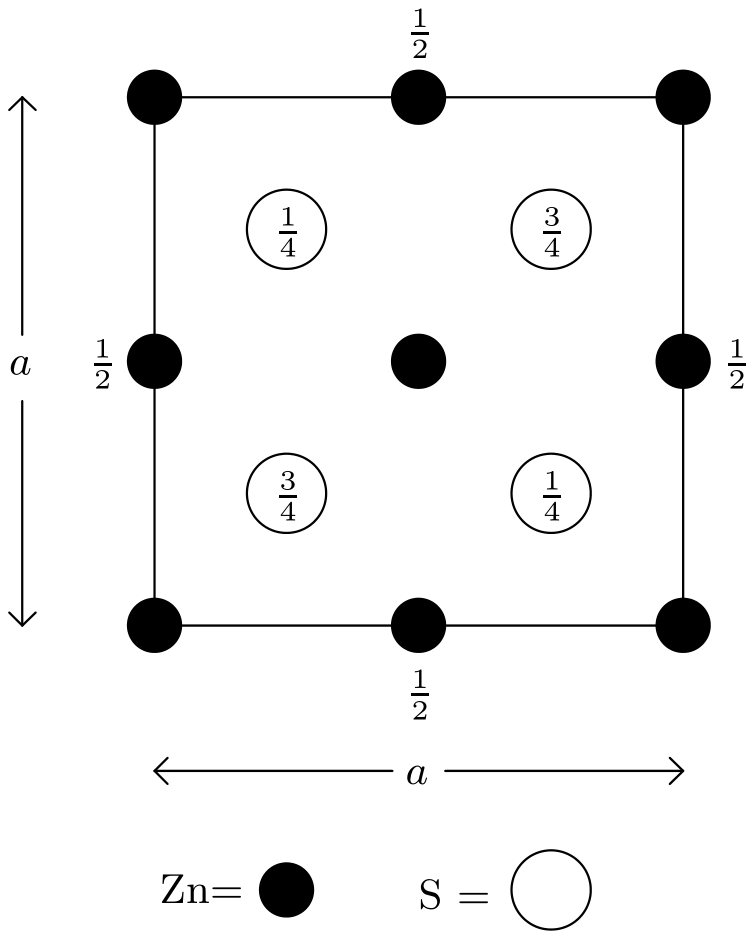
\includegraphics[width=.32\textwidth]{2.png}
        \caption{Plan view of conventional unit cell of zincblende.}
        \label{2}
    \end{figure}
\end{prob}
\begin{sol}
    \begin{enumerate}
        \item[(a)] 该布拉维格子的类型为fcc.
        \item[(b)] 基元可以由处在$[0,0,0]$的Zn原子和处在$[\frac{1}{4},\frac{1}{4},\frac{3}{4}]$的S原子组成.
        \item[(c)] 最近的两个Zn原子间的距离为$\frac{a}{\sqrt{2}}=0.383$nm,一个Zn原子和与之最近的S原子间的距离为$a\sqrt{\left(\frac{1}{4}\right)^2+\left(\frac{1}{4}\right)^2+\left(\frac{1}{4}\right)^2}=0.234$nm,最近的两个S原子间的距离为$\frac{a}{\sqrt{2}}=0.383$nm.
    \end{enumerate}
\end{sol}

\begin{prob}[(12.4) Packing Fractions]
    Consider a lattice with a sphere at each lattice point. Choose the radius of the spheres to be such that neighboring sphere just touch (see for example, Fig. 12.18). The packing fraction is the fraction of the volume of all the space which is enclosed by the union of all the spheres (i.e., the ratio of the volume of the sphere to the total volume).
    \begin{enumerate}
        \item[(a)] Calculate the packing fraction for a simple cubic lattice.
        \item[(b)] Calculate the packing fraction for a bcc lattice.
        \item[(c)] Calculate the packing fraction for an fcc lattice.
    \end{enumerate}
\end{prob}
\begin{sol}
    \begin{enumerate}
        \item[(a)] 简单立方的晶格常数为原子半径的$2$倍,原胞体积为$(2r)^3$,原胞内共有$1$个原子,原子占据的体积为$\frac{4}{3}\pi r^3$,空间利用率为$\frac{\frac{4}{3}\pi r^3}{(2r)^3}=\frac{\pi}{6}\approx 0.52$.
        \item[(b)] 体心立方的晶格常数为原子半径的$\frac{4}{\sqrt{3}}$倍,传统原胞体积为$\left(\frac{4r}{\sqrt{3}}\right)^3$,原胞内共有$2$个原子,原子占据的体积为$2\times\frac{4}{3}\pi r^3$,空间利用率为$\frac{2\times\frac{4}{3}\pi r^3}{\left(\frac{4r}{\sqrt{3}}\right)^3}=\frac{\sqrt{3}}{8}\pi\approx 0.68$.
        \item[(c)] 面心立方的晶格常数为原子半径的$\frac{4}{\sqrt{2}}=2\sqrt{2}$倍,原胞体积为$(2\sqrt{2}r)^3$,原胞内共有$4$个原子,原子占据的体积为$4\times\frac{4}{3}\pi r^3$,空间利用率为$\frac{4\times\frac{4}{3}\pi r^3}{(2\sqrt{2}r)^3}=\frac{\pi}{3\sqrt{2}}\approx 0.74$.
    \end{enumerate}
\end{sol}

\begin{prob}[(12.5) Fluorine Beta Phase]
    Fluorine can crystalize into a so-called beta-phase at temperatures between $45$ and $55$ Kelvin. Fig. 12.23 shows the cubic conventional unit cell for beta phase fluorine in three-dimensional form along with a plan view.
    \begin{figure}[h]
        \centering
        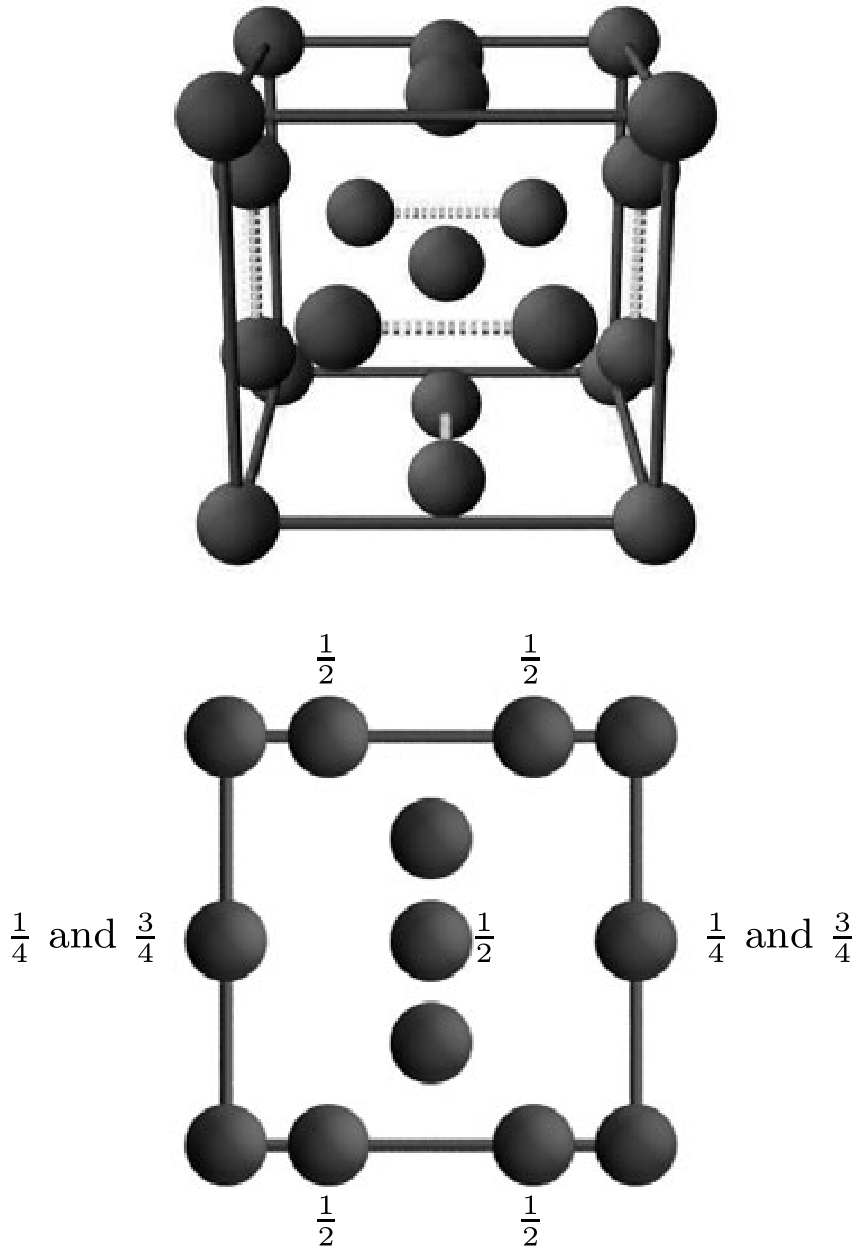
\includegraphics[width=.4\textwidth]{4.png}
        \caption{A conventional unit cell for fluorine beta phase. All atoms in the picture are fluorine. Lines are drawn for clarity \textbf{Top}: Three-dimensional view. \textbf{Bottom}: Plan view. Unlabeled atoms are at height $0$ and $1$ in units of the lattice constant.}
    \end{figure}
    \begin{itemize}
        \item[$\triangleright$] How many atoms are in this conventional unit cell?
        \item[$\triangleright$] What is the lattice and the basis for this crystal?
    \end{itemize}
\end{prob}
\begin{sol}
    \begin{itemize}
        \item[$\triangleright$] 在这一传统原胞中,共有$8\times\frac{1}{8}+12\times\frac{1}{2}+1=8$个原子
        \item[$\triangleright$] 该晶体的格子类型为简单立方,基元可以由位于$[0,0,0]$,$[\frac{1}{4},\frac{1}{2},0]$,$[\frac{3}{4},\frac{1}{2},0]$,$[\frac{1}{2},0,\frac{1}{4}]$,$[\frac{1}{2},0,\frac{3}{4}]$,$[0,\frac{1}{4},\frac{1}{2}]$,$[0,\frac{3}{4},\frac{1}{2}]$,$[\frac{1}{2},\frac{1}{2},\frac{1}{2}]$的$8$个原子组成.
    \end{itemize}
\end{sol}

\begin{prob}[补充题1]
    请利用FCC晶格的传统晶胞证明,FCC晶格是ABC堆垛的六角密排(hexagonal close packing)结构.
\end{prob}
\begin{sol}
    如图\ref{5-fcc-111},从fcc晶格的$[1,1,1]$方向看去,第一层原子($[0,0,0]$这一个原子,标号1)处于第二层原子($[\frac{1}{2},\frac{1}{2},0]$,$[0,\frac{1}{2},\frac{1}{2}]$这三个原子,标号2,3,4)所组成的等边三角形的空隙处,而第三层原子($[\frac{1}{2},\frac{1}{2},1]$,$[1,\frac{1}{2},\frac{1}{2}]$,$[\frac{1}{2},1,\frac{1}{2}]$这三个原子,标号5,6,7)继续堆叠在第二层原子的空隙上,但是第三层原子并不与第一层原子重合,故FCC晶格是ABC堆垛的六角密排.
    \begin{figure}[h]
        \centering
        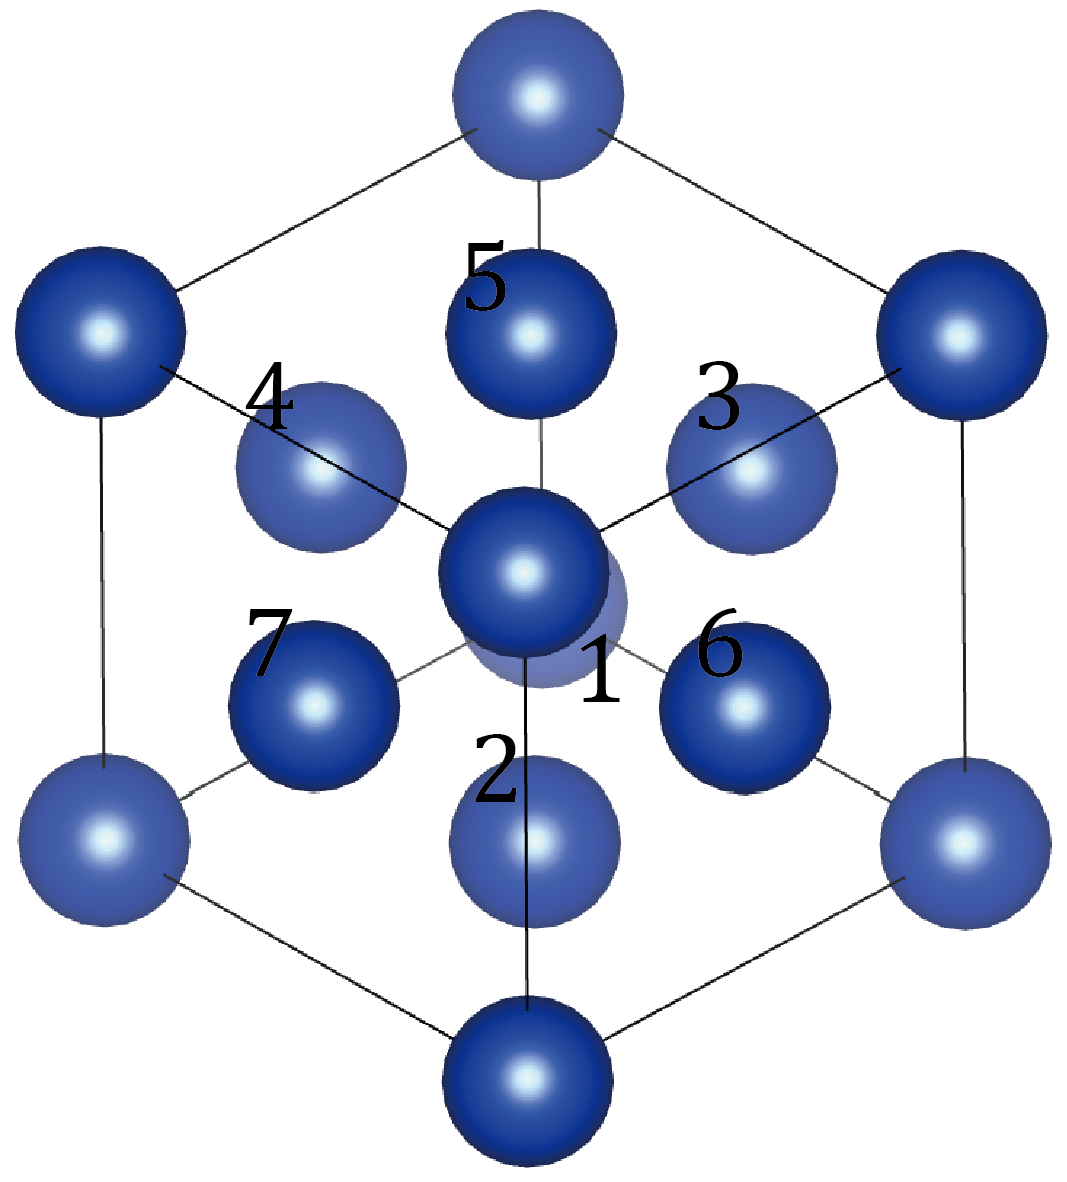
\includegraphics[width=.32\textwidth]{5-fcc-111-2.png}
        \caption{从$[1,1,1]$方向上看到的FCC立方.}
        \label{5-fcc-111}
    \end{figure}
\end{sol}

\begin{prob}[补充题2]
    请证明ABA堆垛的六角密排结构属于hexagonal晶系.
\end{prob}
\begin{sol}
    如图\ref{6-aba-hexagonal}为ABA堆垛的六角密排结构,可以看到其唯一的高次轴为六次反轴(以底面中心原子和底面中心原子所连直线为旋转轴,以中间层等边三角形的中心为对称原点),因此这一结构应当属于hexagonal结构.
    \begin{figure}[h]
        \centering
        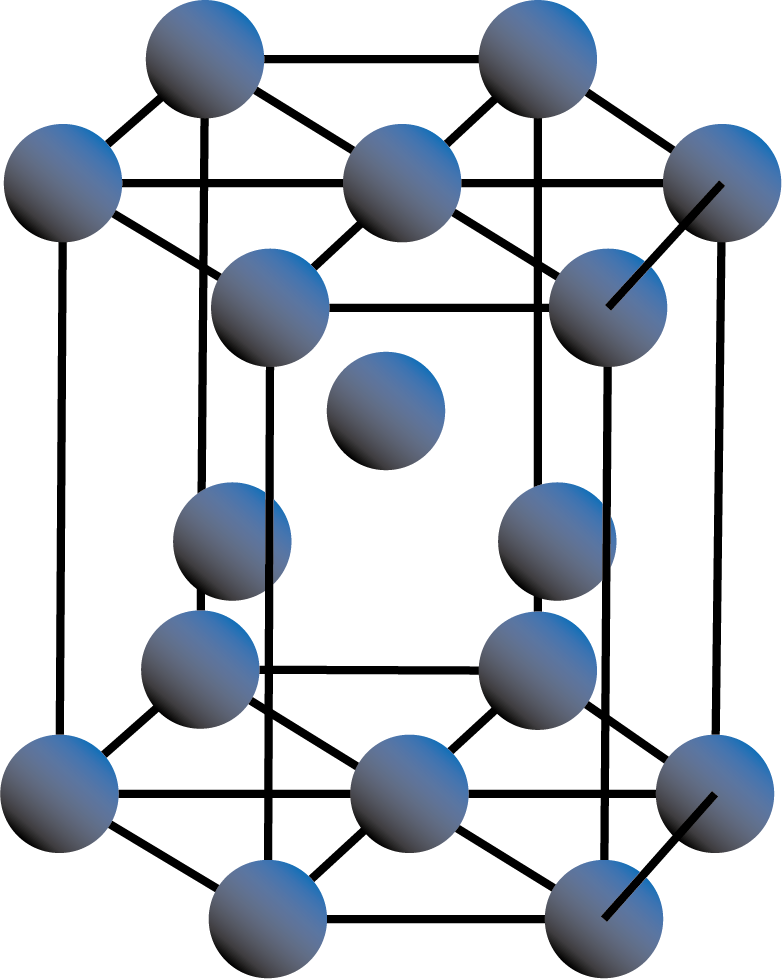
\includegraphics[width=.32\textwidth]{6-aba-hexagonal.png}
        \caption{ABA堆垛的六角密排结构.}
        \label{6-aba-hexagonal}
    \end{figure}
\end{sol}
\end{document}